%%%%%%%%%%%%%%%%%%%%%%%%%%%%%%%%%%%%%%%%%
% Document Author: Hrishikesh R. Gadkari
% Course: CS-734, Fall 2017 at Old Dominion University
%
%
%%%%%%%%%%%%%%%%%%%%%%%%%%%%%%%%%%%%%%%%%
%----------------------------------------------------------------------------------------
%	PACKAGES AND OTHER DOCUMENT CONFIGURATIONS
%----------------------------------------------------------------------------------------

\documentclass{article}

\usepackage{fancyhdr} % Required for custom headers
\usepackage{lastpage} % Required to determine the last page for the footer
\usepackage{extramarks} % Required for headers and footers
\usepackage{listings}
\usepackage{graphicx} % Required to insert images
\usepackage{lipsum} % Used for inserting dummy 'Lorem ipsum' text into the template
\usepackage[bookmarks,bookmarksopen,bookmarksdepth=2]{hyperref} % for bookmarks
\usepackage{enumerate}
\usepackage{csquotes} % for quoting things
\usepackage{multirow}
\usepackage{amsmath}
\usepackage{caption}
\usepackage{navigator}%\usepackage{caption}
\usepackage[shortlabels]{enumitem}
\usepackage{enumitem}
\usepackage{lmodern}
\usepackage[utf8]{inputenc}
%\usepackage[table]{xcolor}% http://ctan.org/pkg/xcolo
\usepackage[dvipsnames]{xcolor}
\usepackage{longtable}
\usepackage{textcomp}
\usepackage{url}
\usepackage{import}
\usepackage{float}
\usepackage{dashrule} % for dashline
\usepackage{keystroke}
\usepackage{amssymb}
\usepackage{booktabs}

\lstdefinestyle{numbers}
{ frame=tb,
  language=python,
  aboveskip=3mm,
  belowskip=3mm,
  showstringspaces=false,
  columns=flexible,
  basicstyle={\small\ttfamily},
  numbers=left,
  numberstyle=\tiny\color{gray},
  keywordstyle=\color{blue},
  commentstyle=\color{OliveGreen},
  stringstyle=\color{purple},
  breaklines=true,
  breakatwhitespace=true,
  tabsize=3
}

\lstdefinestyle{nonumbers}
{ frame=shadowbox,
  language=python,
  aboveskip=3mm,
  belowskip=3mm,
  showstringspaces=false,
  columns=flexible,
  basicstyle={\small\ttfamily},
  numbers=none,
  numberstyle=\tiny\color{gray},
  keywordstyle=\color{blue},
  commentstyle=\color{OliveGreen},
  stringstyle=\color{purple},
  breaklines=true,
  breakatwhitespace=true,
  tabsize=3
}

\lstdefinestyle{mybox}
{
	basicstyle={\small\ttfamily},
    numbers=left,
    numberstyle=\tiny\color{gray},
    stepnumber=1,
    numbersep=5pt,
    showspaces=false, % don't show spaces by adding underscores
    showstringspaces=false, % don't underline spaces in strings
    showtabs=false, % don't show tabs with underscores
    frame=shadowbox,
    tabsize=4,
    captionpos=b,
    breaklines=true,
    breakatwhitespace=false,
  	keywordstyle=\color{blue},
	commentstyle=\color{OliveGreen},
  	stringstyle=\color{purple},    
    rulesepcolor=\color{red!20!green!20!blue!20},
    numberbychapter=false,
    stringstyle=\color{purple},
}


\providecommand{\providehyphenmins}[2]{}

% Margins
\topmargin=-0.45in
\evensidemargin=0in
\oddsidemargin=0in
\textwidth=6.5in
\textheight=9.0in
\headsep=0.25in 

\linespread{1.1} % Line spacing
\newcommand*{\medtau}{\mathbin{\scalebox{1.5}{$\tau$}}}% increase size of tau
\newcommand*{\medn}{\mathbin{\scalebox{1.1}{n}}}% increase size of letter a
\newcommand\multibrace[3]{\rdelim\}{#1}{3mm}[\pbox{#2}{#3}]}

% Set up the header and footer
\pagestyle{fancy}
\lhead{\hmwkAuthorName} % Top left header
\chead{\hmwkShortClass\ (\hmwkClassInstructor\ \hmwkClassTime): \hmwkShortTitle} % Top center header
%\rhead{\firstxmark} % Top right header
\rhead{} % Top right header
\lfoot{\lastxmark} % Bottom left footer
\cfoot{} % Bottom center footer
\rfoot{Page\ \thepage\ of\ \pageref{LastPage}} % Bottom right footer
\renewcommand\headrulewidth{0.4pt} % Size of the header rule
\renewcommand\footrulewidth{0.4pt} % Size of the footer rule

\setlength\parindent{0pt} % Removes all indentation from paragraphs

%----------------------------------------------------------------------------------------
%	DOCUMENT STRUCTURE COMMANDS
%	Skip this unless you know what you're doing
%----------------------------------------------------------------------------------------

% Header and footer for when a page split occurs within a problem environment
\newcommand{\enterProblemHeader}[1]{
\nobreak\extramarks{#1}{#1 continued on next page\ldots}\nobreak
\nobreak\extramarks{#1 (continued)}{#1 continued on next page\ldots}\nobreak
}

% Header and footer for when a page split occurs between problem environments
\newcommand{\exitProblemHeader}[1]{
\nobreak\extramarks{#1 (continued)}{#1 continued on next page\ldots}\nobreak
\nobreak\extramarks{#1}{}\nobreak
}

\newcounter{sub}[section]
\newenvironment{sub}[1][]{\stepcounter{sub}\thesub #1}{ }

\setcounter{secnumdepth}{4} % Removes default section numbers
\newcounter{homeworkProblemCounter} % Creates a counter to keep track of the number of problems
\newcommand{\sectionNumber}{\arabic{homeworkProblemCounter}.\sub }


\newcommand{\homeworkProblemName}{}
\newenvironment{homeworkProblem}[1][Problem \arabic{homeworkProblemCounter}]{ % Makes a new environment called homeworkProblem which takes 1 argument (custom name) but the default is "Problem #"
\stepcounter{homeworkProblemCounter} % Increase counter for number of problems
\setcounter{sub}{0}
\renewcommand{\homeworkProblemName}{#1} % Assign \homeworkProblemName the name of the problem
\
\section{\homeworkProblemName} % Make a section in the document with the custom problem count
\enterProblemHeader{\homeworkProblemName} % Header and footer within the environment
}{
\exitProblemHeader{\homeworkProblemName} % Header and footer after the environment
}

\newcommand{\problemAnswer}[1]{ % Defines the problem answer command with the content as the only argument
\noindent\framebox[\columnwidth][c]{\begin{minipage}{0.98\columnwidth}#1\end{minipage}} % Makes the box around the problem answer and puts the content inside
}

\newcommand{\homeworkSectionName}{}
\newenvironment{homeworkSection}[1]{ % New environment for sections within homework problems, takes 1 argument - the name of the section
\renewcommand{\homeworkSectionName}{#1} % Assign \homeworkSectionName to the name of the section from the environment argument
\subsection{\homeworkSectionName} % Make a subsection with the custom name of the subsection
\enterProblemHeader{\homeworkProblemName\ [\homeworkSectionName]} % Header and footer within the environment
}{
\enterProblemHeader{\homeworkProblemName} % Header and footer after the environment
}
   
%----------------------------------------------------------------------------------------
%	NAME AND CLASS SECTION
%----------------------------------------------------------------------------------------

\newcommand{\hmwkTitle}{\\Assignment\ \#3: \\} % Assignment title
\newcommand{\hmwkShortTitle}{Assignment 3} % Assignment title
\newcommand{\hmwkDueDate}{Thursday,\ November 9,\ 2017} % Due date
\newcommand{\hmwkClass}{CS-734/834 Introduction to Information Retrieval} % Course/class
\newcommand{\hmwkShortClass}{CS-734/834 Intro to IR} % Course/class
\newcommand{\hmwkClassTime}{- Fall 2017} % Class/lecture time
\newcommand{\hmwkClassInstructor}{Dr.  Michael L. Nelson} % Teacher/lecturer
\newcommand{\hmwkAuthorName}{Hrishi Gadkari} % Your name
\newcommand{\hmwkAuthorEmail}{hgadk001@odu.edu} % Your name
%------------------------------------------------------------
% Algorithm declaration
%------------------------------------------------------------
\lstnewenvironment{algorithm}[1][] %defines the algorithm listing environment
{   
    %\refstepcounter{nalg} %increments algorithm number
    \captionsetup{labelsep=colon} %defines the caption setup for: it ises label format as the declared caption label above and makes label and caption text to be separated by a ':'
    \lstset{ %this is the stype
        frame=tB,
        numbers=left, 
        mathescape=true,
        numberstyle=\tiny,
        basicstyle={\small\ttfamily}, 
        keywordstyle=\color{blue}\bfseries\em,
        keywords={,input, output, return, 
                   datatype, function, in, 
                   if, else, for, foreach, 
                   while, write, begin, end, 
        } %add the keywords you want, or load a language as Rubens explains in his comment above.
        numbers=left,
        xleftmargin=.04\textwidth,
        #1 % this is to add specific settings to an usage of this environment (for instnce, the caption and referable label)
    }
}
{}
%----------------------------------------------------------------------------------------
%	TITLE PAGE
%----------------------------------------------------------------------------------------

\title{
\vspace{2in}
\textmd{\textbf{\hmwkClass:\ \hmwkTitle}}\\
\normalsize\vspace{0.1in}\small{Due\ on\ \hmwkDueDate}\\
\vspace{0.1in}\large{\textit{\hmwkClassInstructor\ }}
\vspace{3in}
}

\author{\textbf{\hmwkAuthorName} \\ \hmwkAuthorEmail}
\date{} % Insert date here if you want it to appear below your name

%----------------------------------------------------------------------------------------
%	START OF DOCUMENT
%----------------------------------------------------------------------------------------
\begin{document}

\clearpage\maketitle
\thispagestyle{empty}


\thispagestyle{empty}
\newpage
\setcounter{page}{1}


%----------------------------------------------------------------------------------------
%	Problem 1
%----------------------------------------------------------------------------------------
\begin{homeworkProblem}[Exercise 6.5]% Custom section title
\vspace*{10pt} % Question 
Describe the snippet generation algorithm in Galago. Would this algorithm
work well for pages with little text content? Describe in detail how you would
modify the algorithm to improve it.\\

\subsection*{Answer}
For this question, I downloaded the source code for Galago version 3.10 from https://sourceforge.net/p/lemur/galago/ci/release-3.10/tree/. It is a part of The Lemur Project. The code for the snippet generator can be found in`galago-3.10/core/src/main/java/org/lemurproject/galago/core/index/corpus/SnippetGenerator.java'. The code is as follows: 




\begin{verbatim}

    public String getSnippet(String documentText, Set<String> queryTerms) throws IOException {
    ArrayList<IntSpan> positions = new ArrayList<IntSpan>();
    Document document = parseAsDocument(documentText, positions);
    return generateSnippet(document, positions, queryTerms);
  }





  private Document parseAsDocument(String text, ArrayList<IntSpan> positions) throws IOException {
     Document document = new Document();
     document.text = text;
 
     // Tokenize the document
     TagTokenizer tokenizer = new TagTokenizer();
     tokenizer.process(document);
 
     if (positions != null) {
       positions.addAll(tokenizer.getTokenPositions());
     }
     if (stemming) {
       document = stemmer.stem(document);
     }
 
     return document;
   }



 Private ArrayList<SnippetRegion> findMatches(final Document document, final Set<String> queryTerms) {
     // Make a snippet region object for each term occurrence in the document,
     // while also counting matches
     ArrayList<SnippetRegion> regions = new ArrayList<SnippetRegion>();
 
     for (int i = 0; i < document.terms.size(); i++) {
       String term = document.terms.get(i);
       if (queryTerms.contains(term)) {
         regions.add(new SnippetRegion(term, i, width, document.terms.size()));
       }
     }
     return regions;
   }

  public ArrayList<SnippetRegion> combineRegions(final ArrayList<SnippetRegion> regions) {
     ArrayList<SnippetRegion> finalRegions = new ArrayList<SnippetRegion>();
     SnippetRegion last = null;
     int snippetSize = 0;
     int maxSize = 40;
 
     for (SnippetRegion current : regions) {
       if (last == null) {
         last = current;
       } else if (last.overlap(current)) {
         SnippetRegion bigger = last.merge(current);
 
         if (bigger.size() + snippetSize > maxSize) {
           finalRegions.add(last);
           last = null;
         } else {
           last = bigger;
         }
       } else if (last.size() + snippetSize > maxSize) {
         break;
       } else {
         finalRegions.add(last);
         snippetSize += last.size();
         last = current;
       }
     }
 
     if (last != null && snippetSize + last.size() < maxSize) {
       finalRegions.add(last);
     }
 
     return finalRegions;
   }


 public String buildHtmlString(Snippet best, Document document, ArrayList<IntSpan> positions) {
    StringBuilder builder = new StringBuilder();

    for (SnippetRegion region : best.regions) {
      if (region.start != 0) {
        builder.append("...");
      }
      int startChar = positions.get(region.start).start;
      int endChar = positions.get(region.end - 1).end;
      int start = 0;

      // section string
      String section = document.text.substring(startChar, endChar);

      for (Match m : region.matches) {
        int startMatchChar = positions.get(m.start).start - startChar;
        int endMatchChar = positions.get(m.end - 1).end - startChar;

        String intermediate = stripTags(section.substring(start, startMatchChar));
        builder.append(intermediate);
        builder.append("<strong>");
        builder.append(stripTags(section.substring(startMatchChar, endMatchChar)));
        builder.append("</strong>");
        start = endMatchChar;
      }

      if (start >= 0) {
        builder.append(stripTags(section.substring(start)));
      }

      // terminate matches once we reached a max length.
      int maxSnippetSize = 500;
      if (builder.length() > maxSnippetSize) {
        break;
      }
    }

    if (best.regions.size() > 1 && best.regions.get(best.regions.size() - 1).end != document.terms.
            size()) {
      builder.append("...");
    }
    return builder.toString();
  }

\end{verbatim}
About the algorithm:
Snippet creation is done by the SnippetGenerator class.  This class takes as parameters to it's getSnippet method the document text as a String and a Set of String query terms, and returns a String that is a query-relevant snippet, or summary, of the document.

The snippet generator begins by turning the document text into a list of tokens for processing.  The generator then parses these tokens, looking for query term matches, and when it finds a match, it creates a SnippetRegion object that stores the location within the document where the query term matched, plus five contextual terms preceding and following each term match.  This equates to storing sentence fragments containing query terms.

After collecting all of the regions in the document containing a query term the generator begins constructing the final snippet by adding the SnippetRegions found from the previous step, combining those regions that overlap each other into larger regions, until a final list of SnippetRegions is created with total length in terms is no greater than 40 + the length of the last SnippetRegion added.

With the final list of SnippetRegions the algorithm builds an HTML string containing all the snippets concatenated together for rendering the snippet in a browser while adding \texttt{<strong>} tags around each query term match for emphasis.


\subsection*{Would this algorithm work well for pages with little text content?}
Based on my analysis, I think Galago's snippet algorithm will not work well for pages with little text content. It is because the algorithm works by matching the query terms with the page content. If there is only little content on the page, then the probability to generate a good snippet will also decrease. 
\end{homeworkProblem}

\subsection*{Describe in detail how you would modify the algorithm to improve it}
We need to define a threshold where the amount of text is not enough and then stem our query terms to find other possible terms related in the text. Further we need to expand our query terms to find other possible terms related in the text and then use the stems and expansion results to generate new sentences ranking. Then identify regions where the added terms are more significant and extract and display the result.

\end{homeworkProblem}

%----------------------------------------------------------------------------------------
%	Problem 2
%----------------------------------------------------------------------------------------
\begin{homeworkProblem}[Exercise 6.1]% Custom section title
\vspace*{10pt} % Question
Using the Wikipedia collection provided at the book website, create a sample
of stem clusters by the following process:
	\begin{enumerate}
	\item Index the collection without stemming.
	
	\item Identify the first 1,000 words (in alphabetical order) in the index.
	
	\item Create stem classes by stemming these 1,000 words and recording which
	words become the same stem.
	
	\item Compute association measures (Dice’s coefficient) between all pairs of stems
	in each stem class. Compute co-occurrence at the document level.
	
	\item Create stem clusters by thresholding the association measure. All terms that
	are still connected to each other form the clusters.	
	\end{enumerate}	
Compare the stem clusters to the stem classes in terms of size and the quality (in
your opinion) of the groupings.

\subsection*{Answer}
For indexing the collection,  sorting the index alphabetically, and taking the first 1000 words, I used the following code and stored the words in result.txt.

\begin{verbatim}

import os
import html2text as html2text
import io

import prettyprint as prettyprint

html_files = []
# traverse the directory to list all the html files in the directory
for root, dirs, files in os.walk(os.path.abspath('../articles')):
    for file in files:
        if file.endswith('.html'):
            filepath = os.path.join(root, file)
            html_files.append(filepath)


file_words_index = {}
all_words = set()

# process each html file
for idx, file in enumerate(html_files):
    print('{} of {}. Processing file {}'.format(idx+1, len(html_files), file))
    print('=' * 30)

    # get text only from each file -> remove all tags
    h = html2text.HTML2Text()
    h.ignore_links = True
    text = h.handle(u' '.join([line.strip() for line in io.open(file, "r", encoding="utf-8").readlines()]))

    # get all words from text by splitting by whitespace
    words = [word.lower() for word in text.split() if word.isalpha()]
    all_words |= set(words)
    file_words_index[os.path.basename(file)] = words


# Select 1000 top words
all_words = sorted(list(all_words))
all_words = all_words[:1000]


word_files_index = {}

# Invert words and files
for idx, word in enumerate(all_words):
    print('{} of {}. Processing word {}'.format(idx + 1, len(all_words), word.encode('utf-8')))
    print('=' * 30)

    files = []
    for file, words in file_words_index.items():
        if word in words:
            files.append(file)
    word_files_index[word] = sorted(set(files))


filename = 'result.txt'
with open(filename, 'wb') as f:
    print('Writing to file {}'.format(filename))

    str_word_files_index = prettyprint.pp_str(word_files_index)
    f.write(str_word_files_index)

    print('Done!')


\end{verbatim}

 Inorder to create the stem classes, I used the Krovetz Stemmer. The following code was used to  create stem classes by stemming the 1,000 words and recorded those words which become the same stem in stemmed.csv.

\begin{verbatim}

#!/usr/bin/python
import json
from krovetzstemmer import Stemmer as KrovetzStemmer
import unicodecsv as csv
from prettyprint import prettyprint


# Instantiate krovetz stemmer
krovetz = KrovetzStemmer()


# Read result of 1_index
with open('result.txt', 'rb') as f:
    str_word_files_index = f.read()
    word_files_index =  json.loads(str_word_files_index)

    stem_word_index = {}
    for word, files in word_files_index.items():
        # Stem word using krovetz
        stemmed_word = krovetz.stem(word)

        # Group by stemmed word
        stem_word_index.setdefault(stemmed_word, [])
        stem_word_index[stemmed_word].append(word)


    filename = 'stemmed.csv'
    with open(filename, 'wb') as f:
        print('Writing to file {}'.format(filename))

        writer = csv.writer(f)
        for stemmed_word, words in stem_word_index.items():
            writer.writerow((stemmed_word, ', '.join(words)))

        print('Done!')

\end{verbatim}

Next step is to create the stem clusters using Dice's Coefficient as the term association measure. I applied the Dice's Coefficient formula in the following code to compute the Dice's Coefficient for each pair of terms in every stem classes and the results were stored in coefficient.csv file. 

\begin{verbatim}

#!/usr/bin/python
import json
import nltk as nltk
from tabulate import tabulate
import unicodecsv as csv
from prettyprint import prettyprint



dice_coef_t = 0.01
stem_clusters = []

# Read result of 1_2_index.txt
with open('result.txt', 'rb') as f1:
    word_files_index = json.loads(f1.read())

    # Read result of 3_stemmed_words.csv
    with open('stemmed.csv', 'rb') as f3:
        for stemmed_word, words in csv.reader(f3):
            words = words.split(', ')

            # create bigrams from words
            bigrams = list(nltk.bigrams(words))
            for word_a, word_b in bigrams:
                # Lookup filename in word_files_index
                files_a = word_files_index[word_a]
                files_b = word_files_index[word_b]
                files_a_sliced_b = list(set(files_b) & set(files_a))

                dice_coef = float(2 * len(files_a_sliced_b)) / (len(files_a) + len(files_b))

                if(dice_coef > dice_coef_t):
                    stem_clusters.append((stemmed_word, word_a, word_b, dice_coef))


stem_clusters = sorted(stem_clusters, key=lambda x: x[3], reverse=True)
# print tabulate(stem_clusters, headers=['stemmed_word', 'word_a', 'word_b', 'dice_coef'])

filename = 'coeficient.csv'
with open(filename, 'wb') as f:
    print('Writing to file {}'.format(filename))

    writer = csv.writer(f)
    for stemmed_word, word_a, word_b, dice_coef in stem_clusters:
        writer.writerow((stemmed_word, word_a, word_b, dice_coef))


\end{verbatim}

With a Dice’s coefficient threshold value of 0.1 applied to filter out the weakly-linked stem class elements,
the following are the remaining stem clusters: 

\noindent

accessible	: accessible, accessibility\\	
activate	: activator, activate, activating\\
activate	: activation, activates\\
accelerator	: accelerators, accelerato\\r
abridge	: abridges, abridged\\
accurate	: accurate, accurately\\
address	: addressing, addresses, addressed, address\\
abomination	: abomination, abominationes\\
accept	: accepting, accepted, accept\\
abbreviation	: abbreviation, abbreviations\\
acclaim	: acclaim, acclaimed\\
adaptation	: adaptations, adaptation\\
abrogate	: abrogation, abrogated\\
accrete	: accreting, accrete, accreted\\
acid	: acidic, acids, acid\\
accommodate	: accommodate, accommodated\\
absolute	: absoluter, absolute\\
acceleration	: acceleration, accelerations\\
additional	: additional, additionally\\
acknowledge	: acknowledges, acknowledged\\
addition	: addition, additions\\
accent	: accent, accented\\
actor	: actors, actor\\
access	: access, accessed, accessing, accesso\\
acyltransferase	: acyltransferase, acyltransferases\\
add	: adding, add, added, adds\\
activist	: activist, activists\\
adapt	: adaption, adapt\\
adapt	: adaptive, adapted\\
acre	: acres, acre\\
achieve	: achieves, achieve\\
achieve	: achieving, achieved\\
abstraction	: abstraction, abstractions\\
accompany	: accompany, accompanying\\
activity	: activities, activity\\
accidental	: accidentally, accidental\\
aberration	: aberrations, aberration\\
acronym	: acronym, acronyms\\
academy	: academy, academies\\
acquire	: acquire, acquiring\\
academician	: academician, academicians\\
abut	: abutting, abuts\\
abuse	: abused, abuse\\
accompaniment	: accompaniment, accompaniments\\
actress	: actresses, actress\\
accuse	: accusing, accuses\\
acute	: acute, acutely\\
accumulate	: accumulate, accumulated\\
abugida	: abugidas, abugida\\
abduct	: abducted, abductors\\
achievement	: achievements, achievement\\
accredit	: accrediting, accredited, accreditation\\
accusation	: accusation, accusations\\
account	: accounting, accounted, accounts\\
accident	: accident, accidents\\
actual	: actual, actualized\\
adapter	: adapter, adapters\\
accomplishment	: accomplishment, accomplishments\\
absolve	: absolved, absolve\\
abjad	: abjads, abjad\\
academic	: academic, academically\\
abrupt	: abrupt, abruptly\\
abolition	: abolitionism, abolition\\
act	: acted, act\\
action	: action, actions\\
acoustic	: acoustical, acoustic, acoustically\\
abbey	: abbeys, abbey\\
acquisition	: acquisitions, acquisition\\
abbot	: abbots, abbot\\

\end{homeworkProblem}

%----------------------------------------------------------------------------------------
%	Problem 3
%----------------------------------------------------------------------------------------
\begin{homeworkProblem}[Exercise 6.2]% Custom section title
\vspace*{10pt} % Question 
Create a simple spelling corrector based on the noisy channel model. Use a
single-word language model, and an error model where all errors with the same
edit distance have the same probability. Only consider edit distances of 1 or 2.
Implement your own edit distance calculator (example code can easily be found
on the Web).

\subsection{Answer}
Peter Norvig's noisy channel spelling correction algorithm was used as the basis for this solution.  The \texttt{checker.py} file is uploaded which was created as an implementation of this algorithm. 

The big.txt file was downloaded from Mr. Norvig's website to calculate language model probability function \(P(W)\).  The words in the text file were counted and stored in a map that was compressed and saved on disk using the pickle python library \cite{py:pickle}.\\

\(P(W)\) is calculated with the following formula:

\[P(W) = \frac{C_W}{N}\]

where \(C_W\) is the word count for word \(W\) and \(N\) is the sum of all word counts.\\

\subsection{Output}
Here is some sample output from the checker.py script:

\begin{figure}[h] \label{lab:term-assc-py}
\caption{Sample Output}
\begin{center}
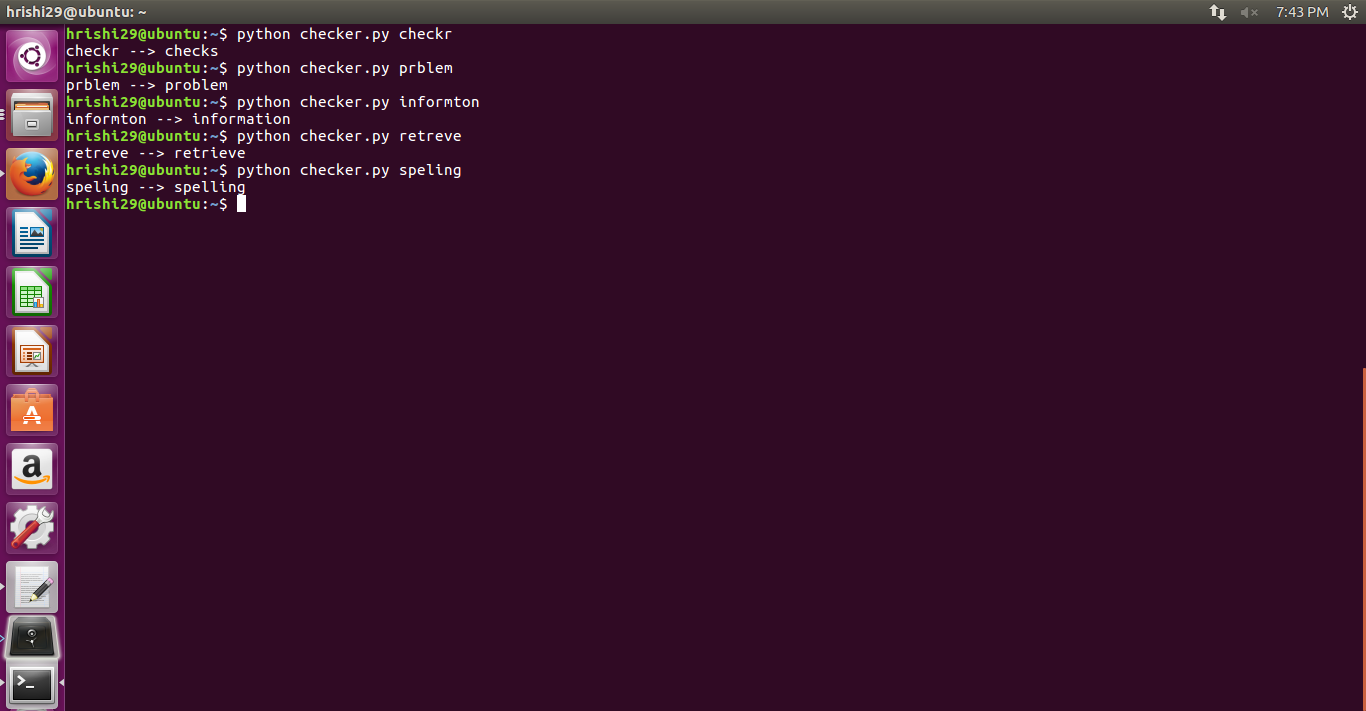
\includegraphics[scale=.40]{sample.png}
\end{center}
\end{figure}

\end{homeworkProblem}

\end{document}